\section{Sharing The Information}
As the network of ubiquitous computers grows bigger, the amount of context information will increase as well and it becomes necessary to understand how this information can be shared. When billions of users and applications is connected to the infrastructure it is important to get the most effective and scalable solution for storing and sharing this kind of data. Applications will need to be able to access the data in real time so the users get the most updated context information. 

As an example scenario we could look at a navigation system in a car. For GPS data to be up to date it needs to be updated when the device moves. A car driving on the highway would travel approximately 30 meters per second. For the positioning system to be accurate the position would need to refresh the location at least once a second, 1 Hz \cite{portas2010validity}. If the location would be shared at the same rate as its refresh rate of 1 Hz it would mean devices would send data every second. This would be a worst case scenario, generally you do not need to update your position if it doesn't change or use a lower refresh rate to compensate for devices moving at a slower speed.

\subsection{Middleware}
To share the information ubiquitous devices need a middleware, a platform that can be run on the ubiquitous devices and enable information sharing. This middleware should be able to provide the functionality for collecting and share context information. The middleware also need to be able to share the context information in real-time. Because of the ubiquitous resource limitations it need to be lightweight and use the resources in an efficient way. This middlewares can share context information in two ways, centralized or decentralized.

\subsection{Centralized}
Centralized middleware solutions are done with a central computer and clients can connect to this computer to store and access context information. In other terms data is hosted and managed in a centralized location, a server, and if a device need to store or access context information it needs to connect to the server. The biggest advantage of the centralized approach is that a server can be updated with new hardware and software to improve its performance. 
A server can only handle a certain amount of requests per second and as the amount of users and applications increase so will the requests to the server. To handle the larger quantities of requests more servers will be needed to share the load and this will cause the costs to scale with the amount of users. Besides not scaling well the centralized approach is more vulnerable to attacks and crashes because when the server goes down users won't be able to retrieve context information. Some examples of internet of things middleware using this approach are SenseWeb \cite{senseweb} and Xively \cite{xively}.

\begin{figure}[t]
	\centering
    	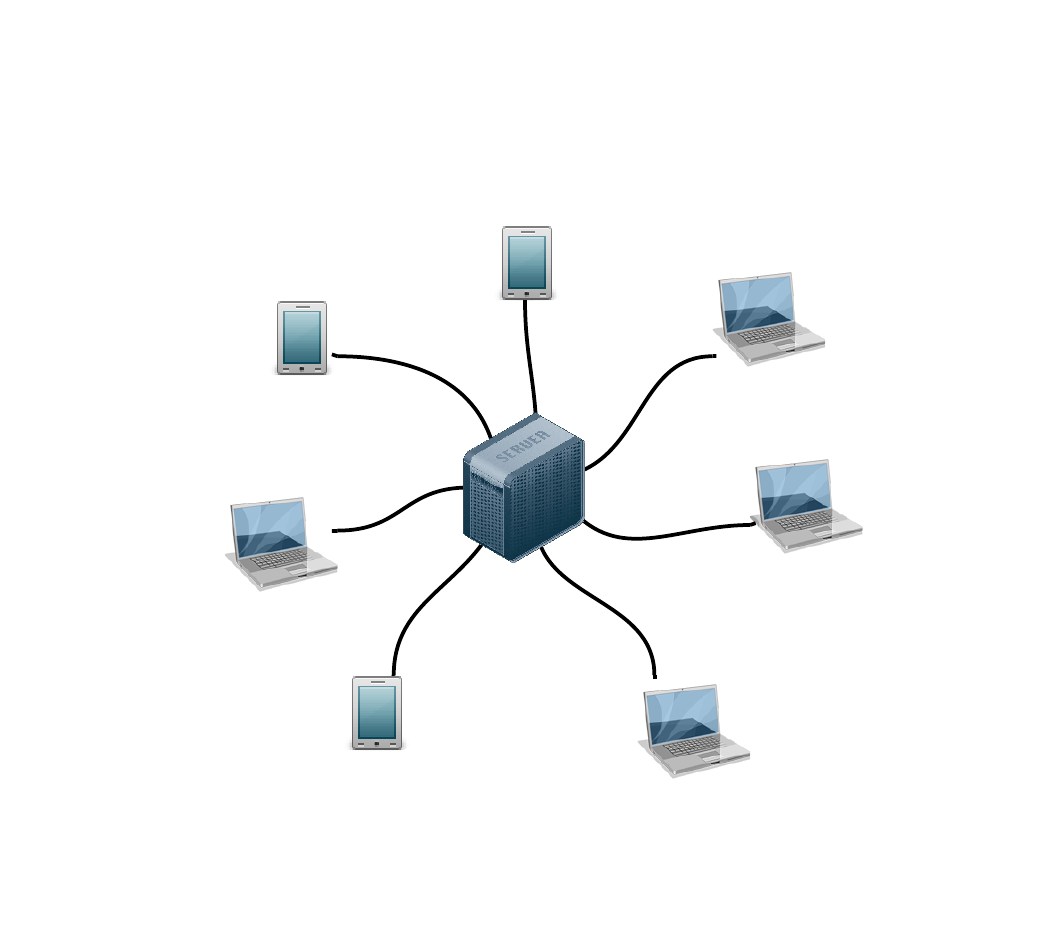
\includegraphics[scale=0.25]{part_2/sharing_the_information/Centralized.png}
		\caption{Overview of a centralized network} 
\end{figure}

\subsection{Decentralized}
In a decentralized network the need for a central server is eliminated. Decentralized networks allow computers / nodes to communicate with each other and to share information and resources without using specialized server computers. Each node in the network has both the server features and the client features. All information is distributed over the network of nodes and not only on a centralized computer. Decentralized networks is a technology that is commonly used in file sharing software applications. A example of file sharing application is that is using this technology is Gnutella. Gnutella is an decentralized search protocol that is used to find files. The benefits of decentralized networks is that the decentralized network is more reliable, the dependency to the server is eliminated. If one node is failing this doesn't affect the other nodes in the network. Another benefit of decentralized network is that attacks to the server is eliminated. In a centralized network the server is vulnerable to Denial-of-service attacks or the server can crash and then the whole network gets affected. Also servers don't need to be updated to new hardware when the network is scaling, so the cost of maintaining decentralized networks is less than centralized networks. Ubiware \cite{osterle2010memorandum} and MediaSense \cite{TheMediaSenseFramework} are both decentralized examples of internet of things middleware. 

\begin{figure}[t]
	\centering
    	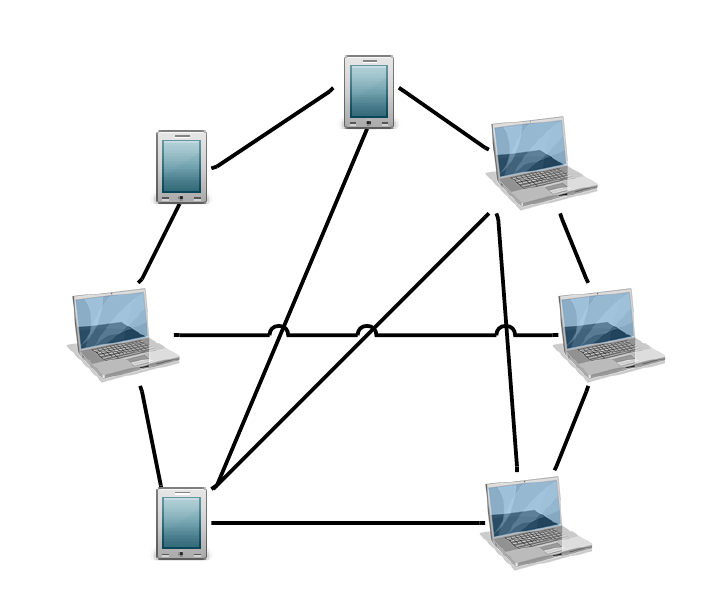
\includegraphics[scale=0.25]{part_2/sharing_the_information/Decentralized.png}
		\caption{Overview of a decentralized network} 
\end{figure}